\documentclass{beamer}

\usepackage[utf8x]{inputenc}
\usepackage{default}
\usepackage{verbatim}
\usepackage{comment}
\usepackage{listings}  
\usepackage{algorithmic}
\usepackage{algorithm}
\usepackage{graphics}

%\usetheme{default}
\usetheme{Boadilla}

\title{Swarm Intelligence Seminar:\\Training Recurrent Neural Network with PSO}
\author{Xiwen Cheng \& Barry van Veen}
\institute{LIACS}
\date{\today}

\begin{document}

\begin{frame}
\titlepage
\end{frame}

\begin{frame}
\tableofcontents
\end{frame}

\section{Goal}
\begin{frame}[fragile]
  \frametitle{Goal}
  \begin{itemize}
    \item To implement a Particle Swarm Optimizer (PSO) and use this to train a Recurrent Neural Network (RNN).
    \item To use the optimized RNN to control a car in a Box2D world
  \end{itemize}  
\end{frame}

\section{Implementation}
\begin{frame}[fragile]
  \frametitle{Implementation}
  \begin{itemize}
    \item C++
    \item Box2D
    \item Using code of last year
  \end{itemize}  
\end{frame}

\begin{frame}[fragile]
  \frametitle{Implementation: PSO}
  \begin{itemize}
    \item Generic PSO
      \begin{itemize}
	\item Neighbourhood: swarm (\textit{global best})
	\item Inertia weight $w$: 0.8
	\item Social parameters: 2.0
	\item $X_{max}$: $[-10, 10]$
	\item $V_{max}$: $[-1, 1]$
	\item Iterations: 100
	\item Particles: 5
      \end{itemize}
  \end{itemize}

  \bigskip
  \begin{tabular}{ll}
    $V(t+1) =$ 	& $w \times V(t)$ \\
		& $+ c_{1} \times rand_{1}() \times (pBest - P(t))$ \\
		& $+ c_{2} \times rand_{2}()\times (nBest - P(t))$ \\
    $P(t+1) =$	& $P(t) + V(t+1)$ \\
  \end{tabular}
\end{frame}

\begin{frame}[fragile]
  \frametitle{Implementation: RNN}
  \begin{itemize}
    \item Fully connected recurrent network
    \item Sigmoid activation function
    \item Input:
      \begin{itemize}
	\item motor speed left wheel
	\item motor speed right wheel
	\item angle of the vehicle
	\item linear velocity
	\item angular velocity right axle
	\item angular velocity left axle
	\item position on y-axis
	\item position on x-axis
	\item position relative to starting point
      \end{itemize}
    \item Output:
      \begin{itemize}
	\item motor speed left wheel
	\item motor speed right wheel
      \end{itemize}
  \end{itemize}
\end{frame}

\begin{frame}[fragile]
  \frametitle{Implementation: putting it all together}

  \begin{columns}
    \begin{column}{0.6\textwidth}
      \begin{itemize}
      \item Evaluation of a particle
	\begin{itemize}
	  \item initialize the Box2D world and RNN
	  \item start loop
	  \begin{itemize}
	    \item extract input from Box2D
	    \item run RNN with inputs
	    \item simulate in Box2d
	  \end{itemize}
	  \item compute fitness (distance traveled)
	\end{itemize}
      \end{itemize}
    \end{column}

    \begin{column}{0.4\textwidth}
    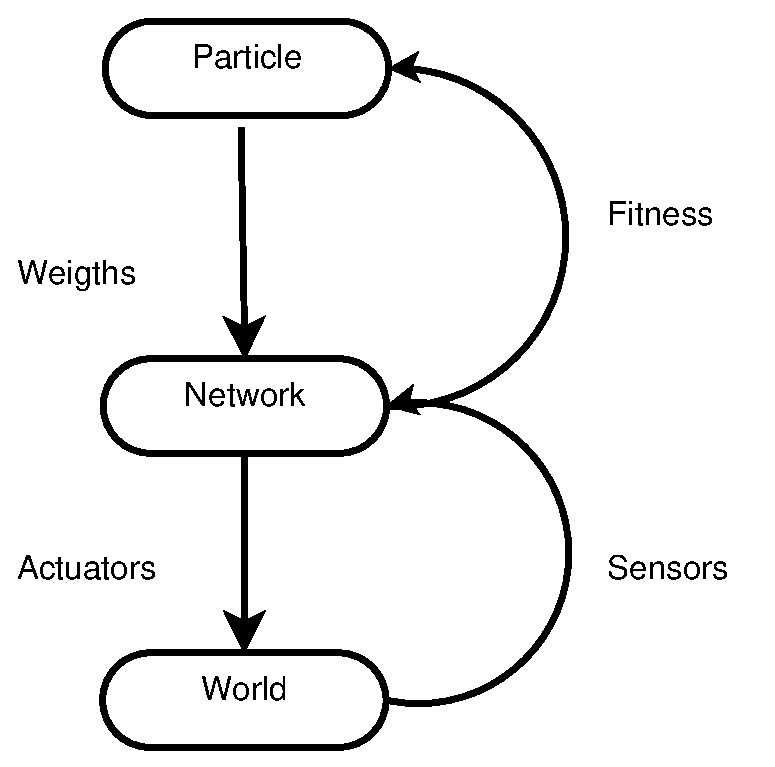
\includegraphics[scale=0.4]{diagram.eps}
    \end{column}

  \end{columns}
\end{frame}



\section{Problems}
\begin{frame}[fragile]
  \frametitle{Problems}
  \begin{itemize}
    \item Implementation of last year
    \item Difficult to connect algorithms to Box2D environment
    \item Hard to tune parameters and quantify results
  \end{itemize}
\end{frame}

\section{Results}
\begin{frame}[fragile]
  \frametitle{Results}
  \begin{itemize}
    \item Our car can overcome obstacles in the world
    \item Multiple worlds tested: good results
  \end{itemize}
\end{frame}

\begin{frame}[fragile]
  \frametitle{Demo}
  Demo!
\end{frame}

\begin{frame}[fragile]
  \frametitle{Further research}
  \begin{itemize}
    \item Robustness
      \begin{itemize}
	\item improve fitness function
	\item NN parameter tuning
	\item training setup (random initialization)
      \end{itemize}
    \item Real time (online) training
  \end{itemize}
\end{frame}

\end{document}
